\documentclass[10pt,twocolumn,letterpaper]{article}

\usepackage{cvpr}
\usepackage[french]{babel}
\usepackage{times}
\usepackage{epsfig}
\usepackage{graphicx}
\usepackage{amsmath}
\usepackage{amssymb}
\usepackage{csquotes}
\usepackage{bm}
\usepackage{mathtools}

% Include other packages here, before hyperref.

% If you comment hyperref and then uncomment it, you should delete
% egpaper.aux before re-running latex.  (Or just hit 'q' on the first latex
% run, let it finish, and you should be clear).
\usepackage[breaklinks=true,bookmarks=false]{hyperref}

\cvprfinalcopy % *** Uncomment this line for the final submission

\def\cvprPaperID{****} % *** Enter the CVPR Paper ID here
\def\httilde{\mbox{\tt\raisebox{-.5ex}{\symbol{126}}}}

% Pages are numbered in submission mode, and unnumbered in camera-ready
%\ifcvprfinal\pagestyle{empty}\fi
\setcounter{page}{1}
\begin{document}

%%%%%%%%% TITLE
\title{Comment tromper les réseaux neuronaux ?}

\author{Adam Hotait\\
CentraleSupélec\\
Deep Learning, Computer Vision\\
{\tt\small adam.hotait@student.ecp.fr}
% For a paper whose authors are all at the same institution,
% omit the following lines up until the closing ``}''.
% Additional authors and addresses can be added with ``\and'',
% just like the second author.
% To save space, use either the email address or home page, not both
\and
Romain Pascual\\
CentraleSupélec\\
Computer Vision\\
{\tt\small romain.pascual@student.ecp.fr}
}

\maketitle
%\thispagestyle{empty}

%%%%%%%%% ABSTRACT
\begin{abstract}
   Nous avons étudié différentes méthodes pour tromper la classification d'un réseau neuronal. Après avoir montré que les réseaux neuronaux étaient robustes à des modifications aléatoires, nous avons mis en œuvre plusieurs méthodes en \og boîte blanche \fg{} permettant de génerer des \textit{adversarial examples} : la méthode FGSM, la méthode FGSM itérative. Nous avons ensuite essayé de cibler quelle classe serait donnée par le réseau neuronal après modification des images.
\end{abstract}

%%%%%%%%% BODY TEXT
\section{Introduction}

L'évolution récente des capacités du Deep Learning, reposant tant sur la disponibilité de données, l'amélioration des connaissances et la démocratisation des puissances de calculs, ouvre la voie à un monde où des algorithmes reposant sur des réseaux neuronaux prendraient des décisions complexes. Ainsi, des réseaux neuronaux pourraient, dans un futur proche, piloter des avions, conduire des voitures, prendre un diagnostic médical ou écrire des articles de presse.

Bien que de nombreux arguments existent aussi bien en faveur qu'en défaveur d'une telle utilisation de la technologie de Deep Learning, arguments qui dépassent pour la plupart le cadre de notre étude, nous avons choisi de nous intéresser à un argument majeur du camp des craintifs : le peu de fiabilité d'un réseau neuronal.

En effet, Szedgy et al. dans leur article \textit{Intriguing properties of neural networks} \cite{szegedy2013intriguing} montrent que les réseaux de neurones sont vulnérables à des \textit{adversarial examples}, c'est à dires des échantillons de données modifiées de manière imperceptible à l'œil humain, mais pouvant duper les réseaux neuronaux.

Goodfellow et. al., dans leur article \textit{Explaining and Harnessing Adversarial Examples} \cite{goodfellow2014explaining} se sont intéressés plus en détail à ces \textit{adversarial examples} et ont générés l'exemple bien connu en Figure \ref{fig:goodfellow_panda}.


%\begin{figure}[t]
%\begin{center}
%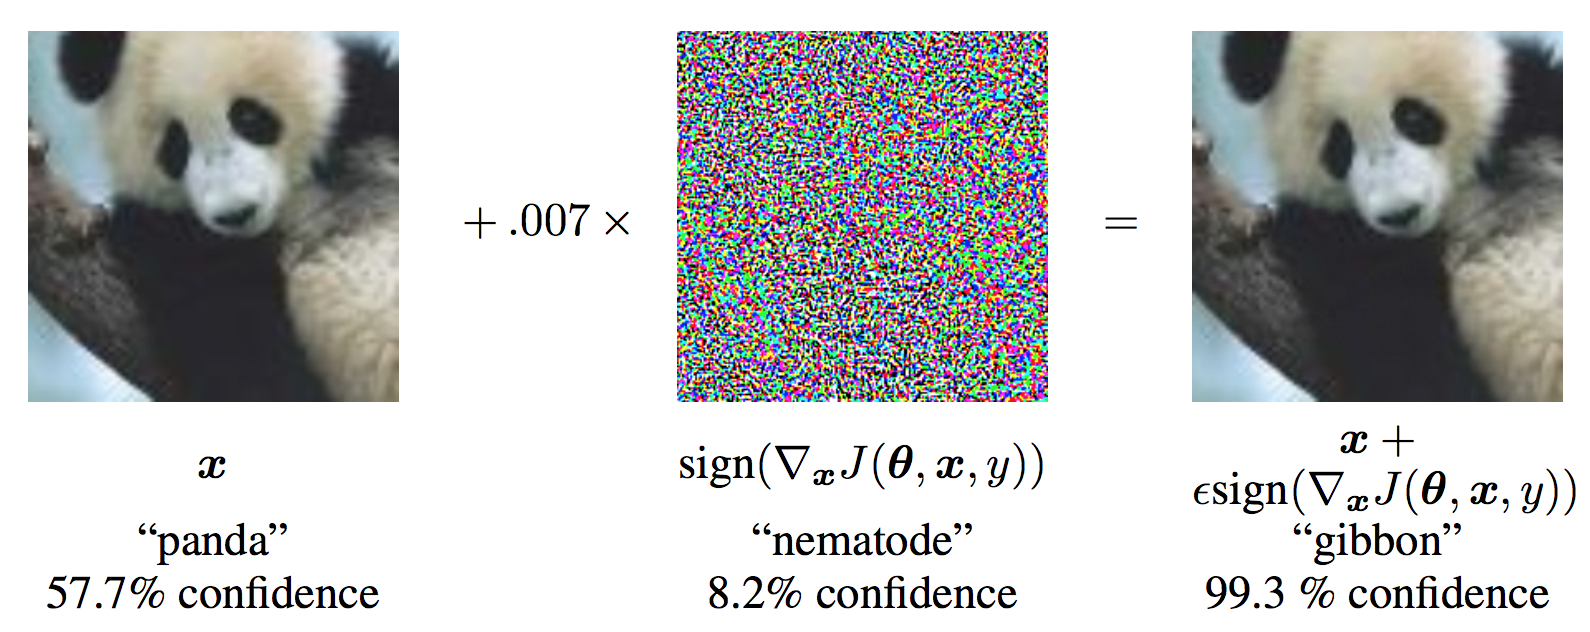
\includegraphics[width=0.8\linewidth]{ressources/goodfellow_panda.png}
%\end{center}
%   \caption{Example of caption.  It is set in Roman so that mathematics
%   (always set in Roman: $B \sin A = A \sin B$) may be included without an
%   ugly clash.}
%\label{fig:long}
%\label{fig:onecol}
%\end{figure}


\begin{figure*}[ht]
\begin{center}
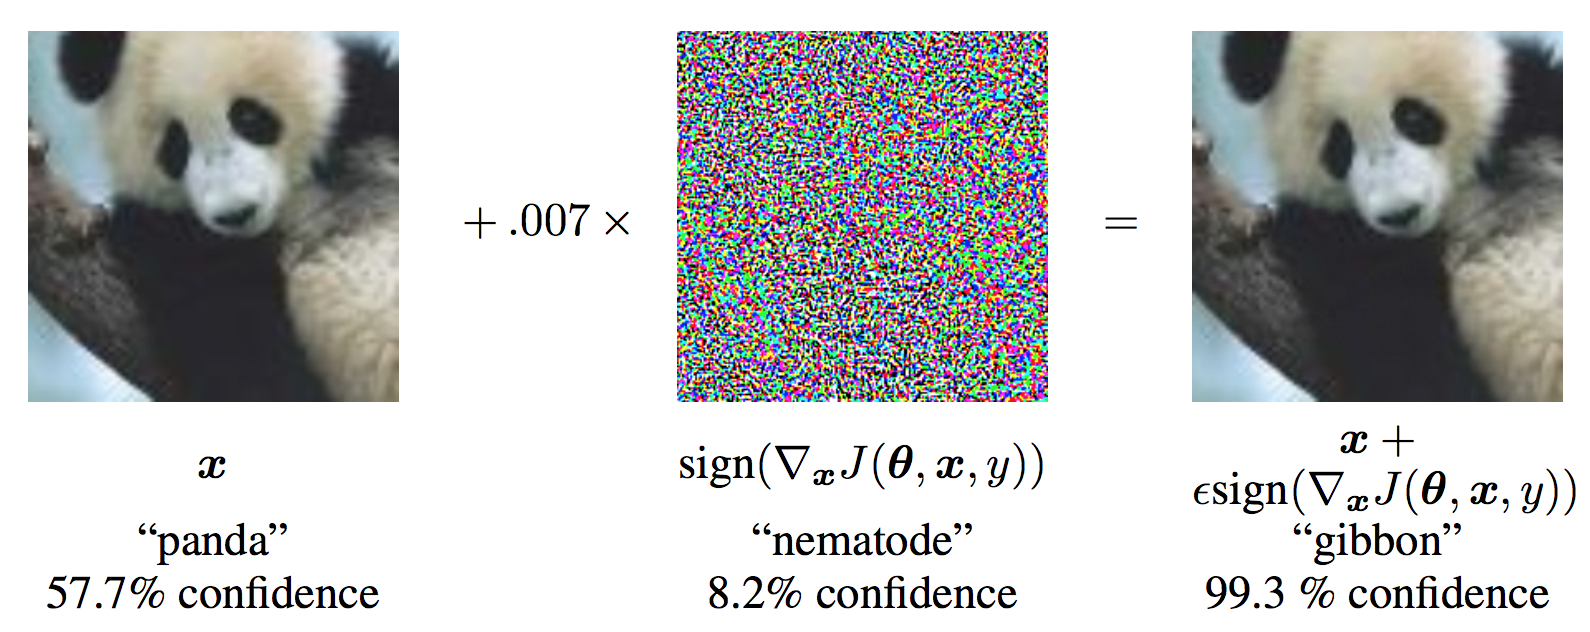
\includegraphics[width=0.8\linewidth]{ressources/goodfellow_panda.png}
\end{center}
   \caption{\textit{Adversarial example} appliqué sur GoogLeNet. À gauche l'image originale classifiée comme un panda, au milieu la perturbation ajoutée avec un poids de 0.007 (invisible à l'oeil humain), à droite l'image modifiée classifiée comme un gibbon.}
\label{fig:goodfellow_panda}
\end{figure*}


Nous pouvons donc nous poser la question de la sécurité des réseaux neuronaux : s'il est simple de modifier une image de manière imperceptible pour conduire à une mauvaise classification, ne serait-il pas possible pour une entité malicieuse de tromper un réseau neuronal, par exemple servant à reconnaissance des routes dans le cadre de la conduite autonome, pour prendre le contrôle du système ?

Afin d'étudier les risques liés aux \textit{adversarial examples}, nous étudierons dans la suite différentes méthodes permettant de tromper un réseau neuronal. Nous commencerons par des méthodes de \textit{misclassification} (dont le but est d'empêcher simplement la bonne classification) puis nous étudierons des méthodes de \textit{target misclassification} (dont le but est de conduire à la classification vers une mauvaise classe choisie).

Notons qu'il existe deux types d'attaques : les attaques en boite blanche, où nous connaissons l'architecture du réseau neuronal attaqué, et les attaques en boite noire, où nous connaissons seulement les entrées et sortie du réseau neuronal attaqué. Bien que les attaques en boite noire soient plus intéressantes car plus génerales, nous allons procéder pour des raisons de simplicité à des attaques en boite blanche.

\section{Réseau neuronal et jeu de données}

Nous utiliserons dans la suite de cette étude le réseau neuronal \textit{ResNet18} \cite{he2016residual}, gagnant de l'ILSVRC (challenge de reconnaissance d'images ImageNet). Nous avons réduit le problème à 8 classes en utilisant le dataset LabelMe, qui contient 2600 images $256 \times 256$ réparties dans les catégories suivantes : autoroute, ville, côte, forêt, immeuble, rue, campagne et montagne \cite{oliva2001modeling}.

La réduction à 8 classes s'est fait par \textit{transfer learning} avec \textit{fine-tuning} de \textit{ResNet18} (batch size de 64, 100 epochs) en s'inspirant du tutoriel à ce sujet sur le site de PyTorch. Nous atteignons une \textit{accuracy} de 0.964815 sur l'ensemble de validation.

Le code correspondant est disponible dans le fichier \texttt{transfer\_learning.py}.

\section{Epsilon}
Le but de cette attaque est de perturber le réseau neuronal en modifiant l'image sans être repéré par l'oeil humain. Dans la figure \ref{fig:diff_epsilon}, nous pouvons voir une image à laquelle nous avons ajouté un masque à plusieurs valeurs différentes de $\epsilon$. Pour des $\epsilon < 0.05$, la perturbation est presque invisible, et elle devient très flagrante pour des $\epsilon > 0.3$.

Le code correspondant est disponible dans le fichier \texttt{epsilon.py}.

\begin{figure}[!ht]
\begin{center}
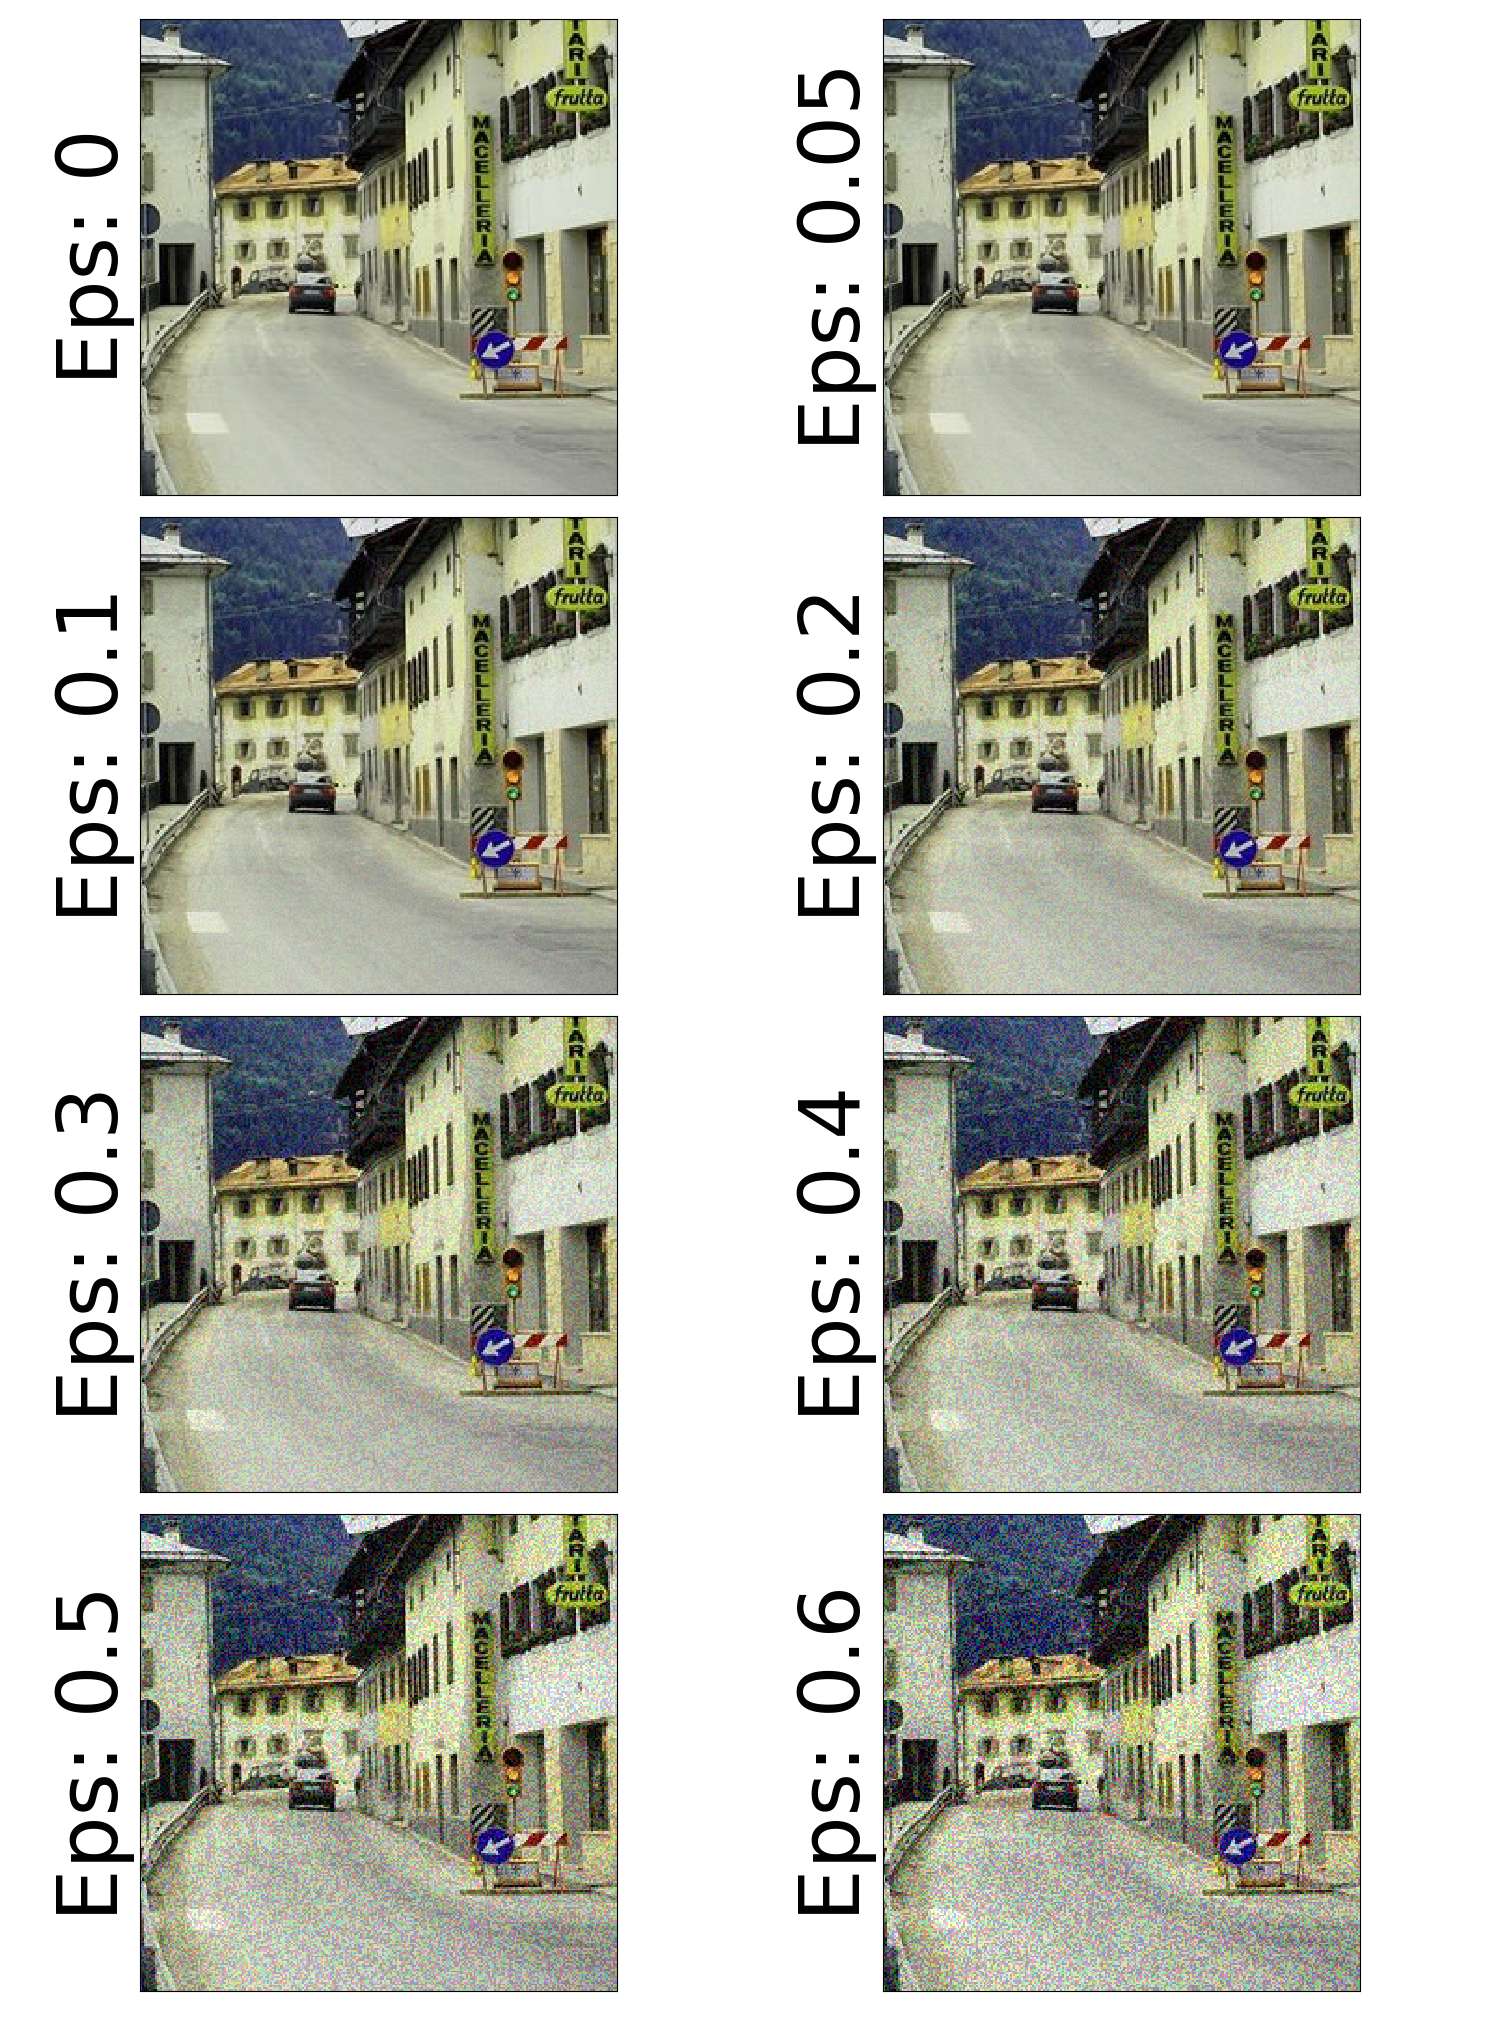
\includegraphics[width=0.9\linewidth]{ressources/epsilon.png}
\end{center}
   \caption{Aspect d'une image modifiée avec un masque aléatoire pour différentes valeurs de $\epsilon$}
\label{fig:diff_epsilon}
\end{figure}

\section{Attaque par bruit aléatoire}

Nous pourrions penser en voyant le bruit ajouté de la Figure \ref{fig:goodfellow_panda} qu'une simple dégradation aléatoire permettrait de dégrader suffisamment l'image pour tromper le réseau neuronal.

Nous avons mis en œuvre l'ajout d'une perturbation aléatoire de nos images avec des $\epsilon$ dans entre 0 et 0.5 en nous inspirant du tutoriel PyTorch sur la géneration d'\textit{adversarial examples} et le dépôt GitHub de l'utilisateur \texttt{sarathknv} \cite{sarath2018}.

Nous voyons cependant dans la Figure \ref{fig:aleatoire_plot} que les réseaux neuronaux sont relativement robustes aux perturbations aléatoires, et ce même si les perturbations sont visibles à l'œil nu comme le montre la figure \ref{fig:aleatoire_img}.

\begin{figure}[!ht]
\begin{center}
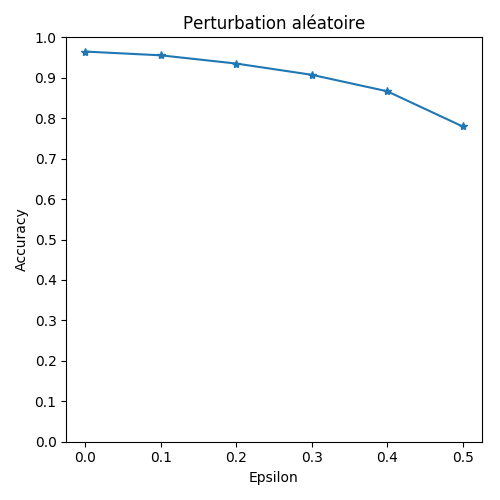
\includegraphics[width=0.85\linewidth]{ressources/aleatoire_plot.png}
\end{center}
   \caption{\textit{Accuracy} du réseau neuronal en fonction de $\epsilon$ pour une perturbation aléatoire}
\label{fig:aleatoire_plot}
\end{figure}

Cela rejoint les conclusions de Goodfellow et al. \cite{goodfellow2014explaining} qui indiquent que :

\begin{displayquote}
La direction de la perturbation, plutôt que le point spécifique de l'espace, est ce qui importe le plus. L'espace n'est pas rempli de poches d'\textit{adversarial examples} qui recouvrent finement les réels comme les nombres rationnels.
\end{displayquote}

\begin{figure}[!ht]
\begin{center}
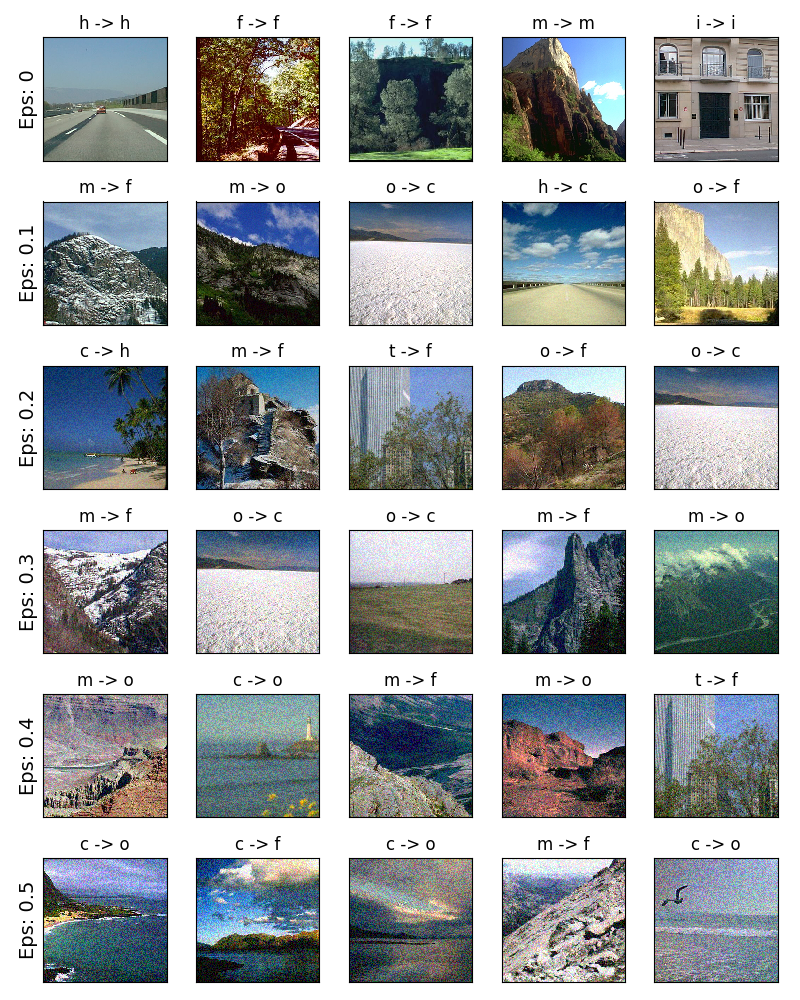
\includegraphics[width=0.9\linewidth]{ressources/aleatoire_img.png}
\end{center}
   \caption{Exemples de perturbation aléatoire trompant le réseau neuronal pour différentes valeurs de $\epsilon$}
\label{fig:aleatoire_img}
\end{figure}

Nous pouvons donc voir qu'il faut bien choisir la perturbation pour espérer tromper un réseau neuronal : une attaque ne saurait consister en une simple dégradation de la qualité d'image.

\section{Fast Gradient Sign Method}

Nous nous intéressons dans cette partie à l'une des premières attaques de réseaux neuronaux, décrite par Goodfellow et al.  \cite{goodfellow2014explaining}, la \textit{Fast Gradient Sign Attack} (attaque rapide du signe du gradient).

L'idée est simple : les réseaux neuronaux fonctionnant par minimisation de la fonction de coût lors de la descente de gradient, l'attaque cherche à modifier l'image de manière à ce que le coût soit maximisé.

C'est cette attaque qui est mise en œuvre dans la Figure \ref{fig:goodfellow_panda} où $\nabla_x J(\bm{\theta}, \bm{X}, y))$ représente alors le gradient de la fonction de coût $J$ utilisée pour entrainer le réseau. Nous connaissons la fonction de coût initiale, cette attaque est donc bien une attaque \og boîte blanche \fg{}.

Soient $\bm{x}$ et $\bm{x}^adv$ respectivement l'image d'origine et un \textit{adversarial example} associé. On a alors l'attaque suivante :

\begin{equation}
\bm{x}^{adv} = \bm{x} + \epsilon sign(\nabla_x J(\bm{\theta}, \bm{x}, y))
\end{equation}

Nous avons mis en œuvre une telle attaque en nous inspirant du tutoriel PyTorch sur la génération d'\textit{adversarial examples} déja utilisé plus haut. Notre domaine de $\epsilon$ s'étend de 0 à 0.03 (un ordre de grandeur de moins que pour les perturbations aléatoires). Le code correspondant est disponible dans \texttt{fgsm\_pert.py}

Le graphique de l'\textit{accuracy} en fonction de $\epsilon$  en figure \ref{fig:fgsm_plot} nous montre que, même avec d'infimes perturbations, le réseau neuronal perd énormément en précision.

\begin{figure}[!h]
\begin{center}
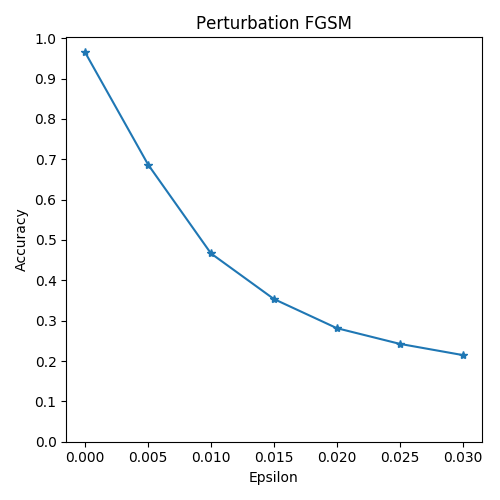
\includegraphics[width=0.85\linewidth]{ressources/fgsm_plot.png}
\end{center}
   \caption{\textit{Accuracy} du réseau neuronal en fonction de $\epsilon$ pour la méthode FGSM}
\label{fig:fgsm_plot}
\end{figure}

Nous avons des exemples d'images modifiées avec succès en figure \ref{fig:fgsm_img}.

\begin{figure}[!h]
\begin{center}
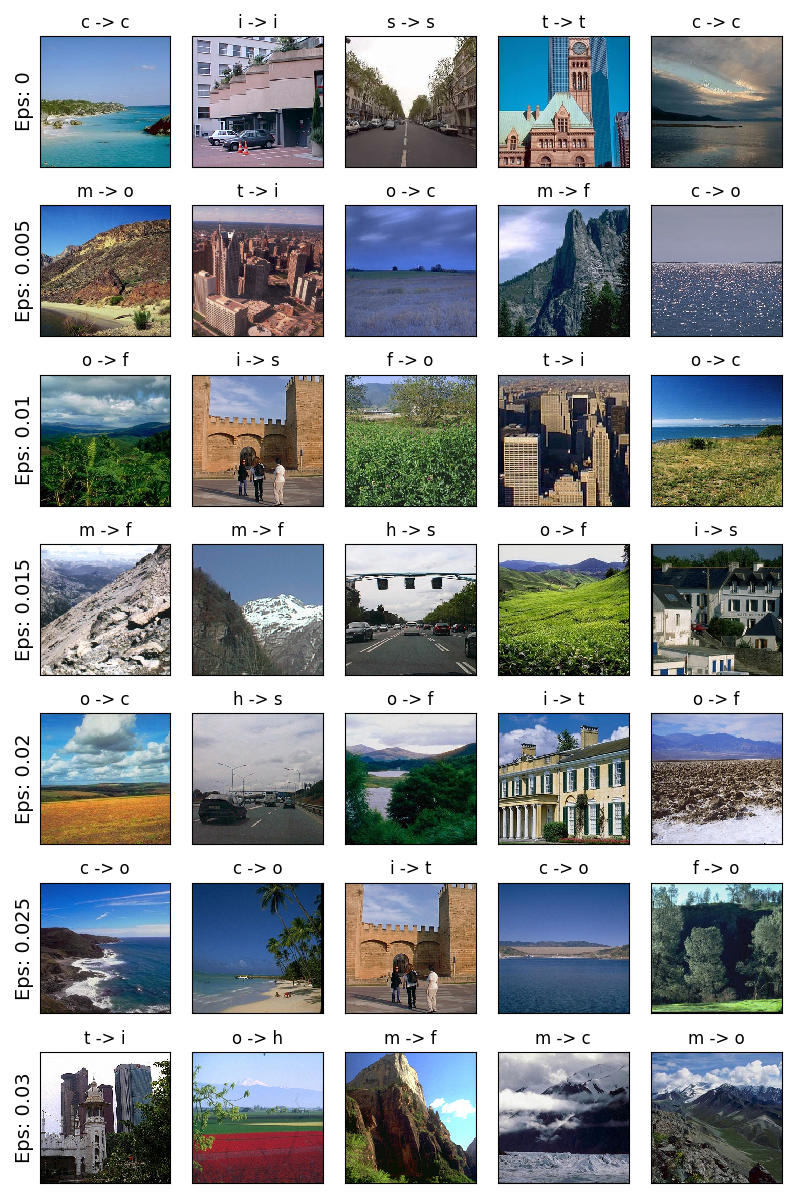
\includegraphics[width=0.9\linewidth]{ressources/fgsm_img.png}
\end{center}
   \caption{Exemples de perturbation FGSM trompant le réseau neuronal pour différentes valeurs de $\epsilon$}
\label{fig:fgsm_img}
\end{figure}

Les limites de cette méthode sont doubles : 
\begin{enumerate}
\item c'est une attaque en boîte blanche, il faut en effet connaitre l'architecture du modèle attaqué, et notamment sa fonction de coût ;
\item c'est une attaque qui va réussir à mal classifier les données, mais qui ne va pas permettre de choisir la classe cible.
\end{enumerate}

\section{Iterative Fast Gradient Sign Method}
Une amélioration de la méthode FGSM est la méthode FGSM itérative \cite{kurakin2016}. Cette attaque consiste à avancer plusieurs fois dans la direction du gradient en s'assurant que chaque pixel reste dans un voisinage de l'image d'origine.

En posant $Clip$ la fonction qui s'assure que nous restons dans le voisinage (pixel à pixel) de l'image d'origine par seuillage, on a :

\begin{align}
\bm{x}^{adv}_0 &= \bm{x}  & \bm{x}^{adv}_{n+1} &= Clip_{x, \epsilon} \Big\{ \bm{x}^{adv}_n +\alpha \nabla_x J(\bm{\theta}, \bm{x}^{adv}_n, y)) \Big\}
\end{align}

Le résultat de l'implémentation de cette méthode (adapté des implémentations précédentes) est disponible sur la figure \ref{fig:fgsm_iter_plot}. Nous pouvons voir que la méthode itérative est plus efficace que la méthode FGSM simple, car elle réussit à tromper le réseau de manière plus significative pour des perturbations de même poids.

\begin{figure}[!h]
\begin{center}
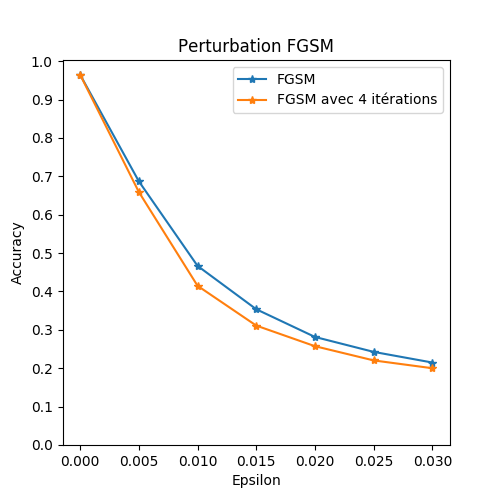
\includegraphics[width=0.85\linewidth]{ressources/fgsm_iter_plot.png}
\end{center}
   \caption{\textit{Accuracy} du réseau neuronal en fonction de $\epsilon$ pour la méthode FGSM itérative. Nous avons choisi $N=4$ itérations et $\alpha =1$.}
\label{fig:fgsm_iter_plot}
\end{figure}

L'attaque est donc plus efficace que le FGSM, au détriment d'un temps de calcul (lié aux $N$ itérations) plus élevé. Elle conserve cependant les deux défauts de FGSM que nous avons identifié.

Le code de cette attaque est disponible dans le fichier \texttt{iterative\_pert.py}

\section{Attaque ciblée}

Un inconvénient majeur des attaques que nous avons étudié (FGSM et FGSM itérative) est l'impossibilité de choisir la classe cible.

Nous pouvons tenter de corriger cela en modifiant l'attaque ainsi pour FGSM :

\begin{equation}
\bm{x}^{adv} = \bm{x} - \epsilon sign(\nabla_x J(\bm{\theta}, \bm{x}, y_{cible}))
\end{equation}

Et pour FGSM itérative :

\begin{align}
\bm{x}^{adv}_0 &= \bm{x}  & \bm{x}^{adv}_{n+1} &= Clip_{x, \epsilon} \Big\{ \bm{x}^{adv}_n -\alpha \nabla_x J(\bm{\theta}, \bm{x}^{adv}_n, y_{pred}) \Big\}
\end{align}

Ainsi, intuitivement, au lieu de chercher à aller contre le sens de la descente de gradient en maximisant le coût de la prédiction classe cible, on cherche à minimiser le coût de la prédiction de la classe cible. Pour le choix de la classe cible, nous pouvons choisir la classe que nous désirons. Deux méthodes courantes de sélection de la classe cible sont l'aléatoire ou le choix de la classe la moins susceptible d'être choisie par le réseau pour l'image attaquée \cite{kurakin2016}.

\subsection{Attaque avec une cible prédéfinie}

Les figures \ref{fig:fgsm_tget_plot} et \ref{fig:fgsm_tget_img} nous montrent les résultats d'une implémentation de l'attaque FGSM sans itération avec comme cible la classe \texttt{mountain}, choisie arbitrairement.

\begin{figure}[!hb]
\begin{center}
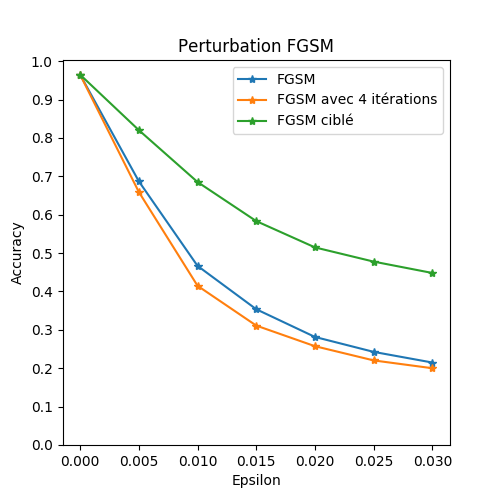
\includegraphics[width=0.85\linewidth]{ressources/fgsm_tget_plot.png}
\end{center}
   \caption{\textit{Accuracy} du réseau neuronal en fonction de $\epsilon$ pour les différentes méthodes FGSM.}
\label{fig:fgsm_tget_plot}
\end{figure}

\begin{figure}[!hb]
\begin{center}
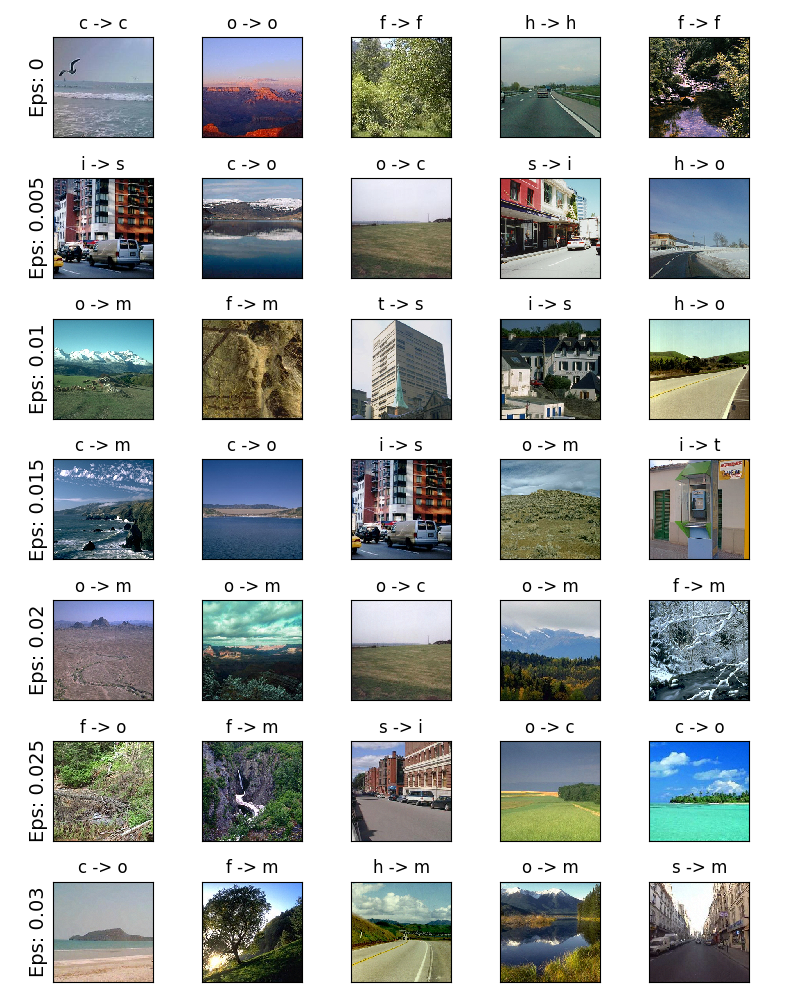
\includegraphics[width=0.85\linewidth]{ressources/fgsm_tget_img.png}
\end{center}
   \caption{Exemples de perturbation FGSM ciblant sur la classe \texttt{mountain} trompant le réseau neuronal pour différentes valeurs de $\epsilon$. Nous pouvons remarquer que toutes les classes des \textit{adversarial examples} ne sont pas \texttt{mountain}.}
\label{fig:fgsm_tget_img}
\end{figure}

Nous pouvons tout d'abord voir que l'\textit{accuracy} du réseau neuronal après cette attaque est réduite. Cela est dû à deux choses :

\begin{enumerate}
\item Les images de la classe \texttt{mountain} sont correctement classées, ce qui diminue forcément l'\textit{accuracy} même s'il n'y avait pas de diminution sur les autres classes.
\item L'attaque se fait en \og allant dans la direction \fg{} de la classe cible. La classe cible étant arbitraire, cela n'est à priori pas aussi efficace qu'aller \og dans la direction opposée \fg{}  à la classe d'origine.
\end{enumerate}

L'attaque classe t-elle l'image dans la classe cible ? Nous pouvons voir sur la figure \ref{fig:fgsm_tget2_plot}, qui représente le taux d'images classées comme \texttt{mountain} en fonction de $\epsilon$, que bien qu'il y a de plus en plus de classification dans la classe \texttt{mountain} avec l'augmentation de $\epsilon$, toutes les mauvaises classifications ne se font pas dans cette classe.

Nous pouvons voir des exemples de mauvaise classification avec la classe résultante sur la figure \ref{fig:fgsm_tget_img}.

\begin{figure}[!h]
\begin{center}
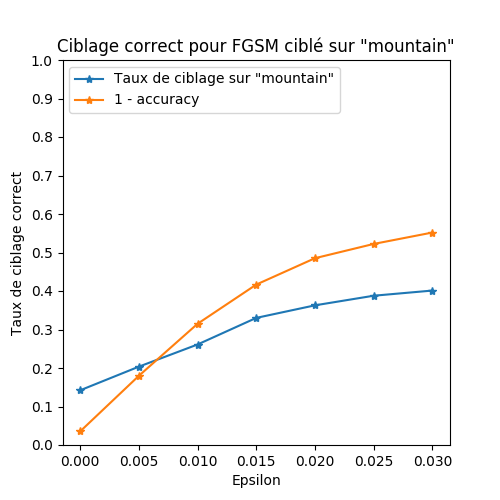
\includegraphics[width=0.85\linewidth]{ressources/fgsm_tget2_plot.png}
\end{center}
   \caption{Taux de ciblage correct pour une attaque FGSM ciblant sur la classe \texttt{mountain}}
\label{fig:fgsm_tget2_plot}
\end{figure}

\subsection{Attaque sur la least-likely class}
Cette attaque vise à cibler la classe ayant la plus petite probabilité de représenter notre image d'origine.

Une implémentation de cette méthode donne les résultats des figures \ref{fig:fgsm_least_plot} et \ref{fig:fgsm_least2_plot}.

Nous voyons que la FGSM ciblée \textit{least-likely} et la FGSM ciblée sur une classe arbitraire on des résultats similaires. Cependant, pour les valeurs de $\epsilon$ testées, nous voyons qu'il y a en fait très peu d'images modifiées qui sont classifiées dans la \textit{least-likely class}.

\begin{figure}[!h]
\begin{center}
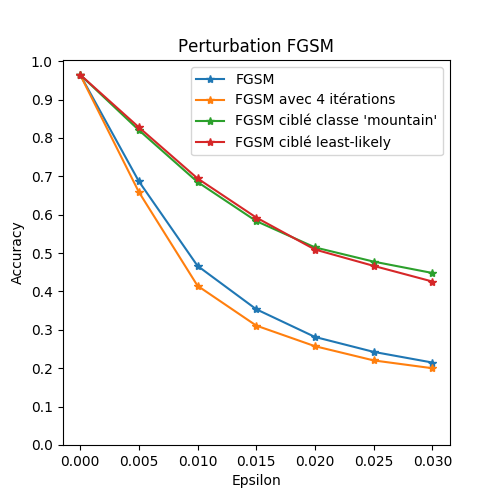
\includegraphics[width=0.85\linewidth]{ressources/fgsm_least_plot.png}
\end{center}
   \caption{\textit{Accuracy} du réseau neuronal en fonction de $\epsilon$ pour les différentes méthodes FGSM.}
\label{fig:fgsm_least_plot}
\end{figure}

\begin{figure}[!h]
\begin{center}
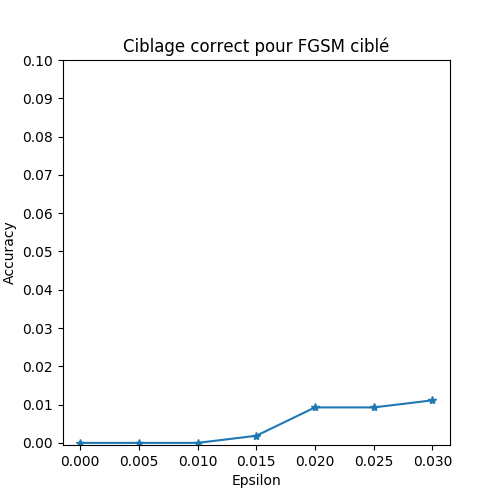
\includegraphics[width=0.85\linewidth]{ressources/fgsm_least2_plot.png}
\end{center}
   \caption{Taux de ciblage correct pour une attaque FGSM ciblant sur la \textit{least-likely class}. Notez la différence d'échelle par rapport à la figure \ref{fig:fgsm_tget2_plot}.}
\label{fig:fgsm_least2_plot}
\end{figure}

\subsection{Code}

Le code est disponible dans \texttt{fgsm\_target\_pert.py}. Nous avons aussi écrit une méthode itérative ciblée dans \texttt{iterative\_target\_pert.py}.
\section{One Pixel Attack}

Les perturbations que nous avons étudiée est facilement détectable : la méthode de perturbation étant l'ajout à l'image d'un bruit (bien que spécifique), des méthodes de réduction de bruit peuvent permettre de se prémunir d'une telle attaque \cite{liang2018}.

Il existe cependant d'autres manières de génerer des \textit{adversarial examples}. L'une d'entre elle, baptisée \textit{One Pixel Attack}, vise à modifier seulement quelques pixels bien choisis \cite{su2019}.

Nous avons essayé de mettre en œuvre cette méthode dans le fichier \texttt{onepixel\_pert.py} en nous inspirant du code de l'utilisateur GitHub \texttt{sarathknv} \cite{sarath2018}. Cependant, l'attaque initiale était effectuée sur le jeu de donnée CIFAR-10 \cite{krizhevsky2009}, qui est constituée d'images $32\times 32$. Notre jeu de données étant une base d'images $256\times 256$ (il faut donc modifier plus de pixels pour réussir l'attaque) et la méthode étant basée sur un algorithme d'évolution différentielle, très couteuse en ressources, nous n'avons pas pu tester notre implémentation avec succès.

\section{Pour aller plus loin}
Pour aller plus loin, les pistes d'amélioration suivantes sont proposées :

\begin{itemize}
\item Nous avons été grandement limités par la puissance de calcul  et le temps disponible (scripts lancés sur un MacBookPro sur un CPU Intel Core i5 @ 2.3GHz). Il serait souhaitable de mener les mêmes études sur des domaines de variables plus étendus ($\epsilon, \alpha$ ou nombre d'itérations par exemple).
\item Nous avons étudiés des méthodes d'attaque (génération d'\textit{adversarial examples}), il serait souhaitable d'étudier aussi des méthodes de défense (ne pas se faire tromper par des \textit{adversarial examples}).
\item Nous avons étudié des méthodes d'attaque en \og boîte blanche \fg{}. Nous n'avons pas toujours accès à l'architecture des réseaux neuronaux, il serait donc souhaitable d'étudier des méthodes d'attaque en \og boîte noire \fg{}.
\item Nous souhaiterions mettre en place d'autres méthodes, dont des GANs.
\item Sur un plan plus pragmatique, il serait souhaitable de procéder à un nettoyage de notre code.
\end{itemize}

\section{Conclusion}
Nous avons étudié plusieurs méthodes de génération d'\textit{adversarial examples}.
Plusieurs points ont été évoqués :
\begin{itemize}
\item Les \textit{adversarial examples} ne sont pas un simple ajout de bruit aléatoire.
\item Une méthode rapide pour générer un \textit{adversarial example} et la manipulation de la manière dont fonctionne un réseau neuronal : la minimisation d'une fonction de coût. Si on connait l'architecture du réseau, on peut manipuler notre image afin d'augmenter le coût de la classe d'origine.
\item Il est possible de choisir quelle mauvaise classe va être choisie par le réseau neuronal pour une image donnée. Ces méthodes sont cependant moins performantes qu'un simple FGSM.
\end{itemize}

{\small
\bibliographystyle{unsrt}
\bibliography{dlcv}
}

\end{document}
